\documentclass[12pt]{article}

% ---------------------------------------------------------------------------
% Preamble
% ---------------------------------------------------------------------------
\usepackage[T2A]{fontenc}
\usepackage[utf8]{inputenc}
\usepackage[russian]{babel}
\usepackage[margin=2.5cm]{geometry}
\usepackage{graphicx}
\usepackage{hyperref}

\hypersetup{
  colorlinks=true,
  linkcolor=blue!50!black,
  urlcolor=blue!50!black,
  citecolor=blue!50!black
}

\title{Вложение нескольких конечных автоматов в одно состояние:\\
доработка алгоритма умножения на примере счётчика джекпота}
\author{}
\date{\today}

\begin{document}
\maketitle

\noindent
\textbf{Цель работы:} улучшить существующий алгоритм умножения конечных
автоматов так, чтобы он корректно поддерживал вложение нескольких
независимых автоматов в одно и то же состояние родителя, и продемонстрировать
это на реальной модели: добавить в систему «игровой автомат» новый
автомат-компонент счётчик джекпота, вложенный наравне с уже существующим
автоматом барабанов в состояние «Игра».

До этой работы алгоритм уже умел умножать пару автоматов и раскрывать один
уровень вложенности (например, барабаны $A_2$, вложенные в состояние
«Игра» автомата $A_0$). Задача требует другого случая --- двух вложенных
автоматов в одно и то же состояние одновременно, где один из них должен
опираться на внутреннее состояние другого. Этот случай потребовал
модернизировать сам алгоритм умножения. Теперь в процессе умножения
автоматы помнят «родные» состояния каждого вложенного автомата даже после
слияния в общий автомат. Раньше проверка «автомат сейчас в таком-то
состоянии» работала только пока автоматы ещё не объединили: как только
несколько автоматов сливались в один большой, старые номера состояний
терялись, и проверка переставала быть верной.

\section{Дополненная система конечных автоматов}

Система «игровой автомат» дополнена новым вложенным автоматом «счётчик
джекпота». Ниже приведены диаграмма состояний и таблица входных/выходных
событий для каждого из четырёх автоматов, а также для итогового
перемноженного автомата.

\subsection*{Автомат 1. «Игровая машина» ($A_0$)}

\begin{figure}[h]
\centering
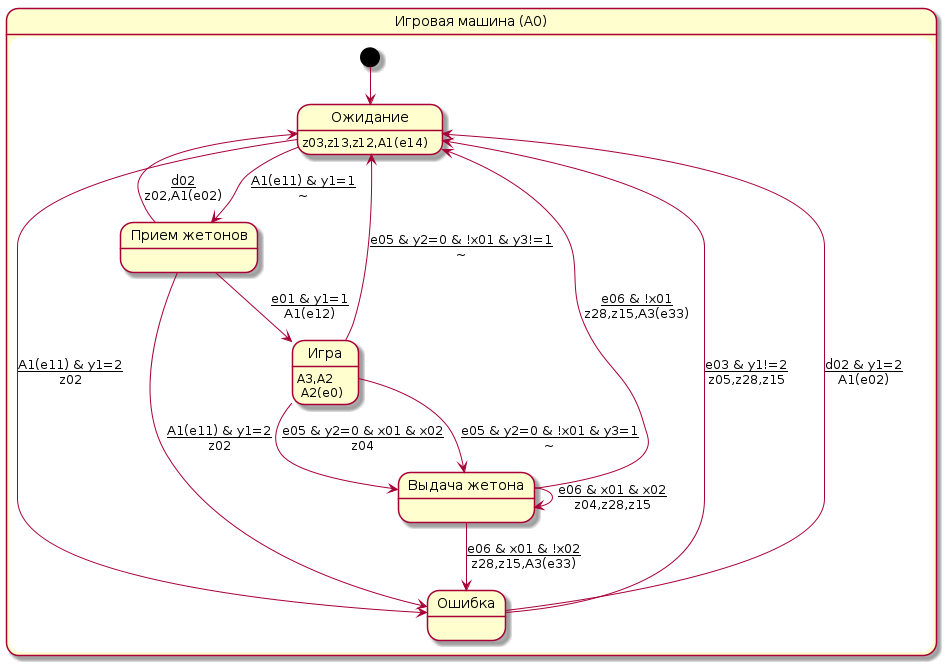
\includegraphics[width=0.95\textwidth]{images/a0_diagram.png}
\caption{Диаграмма состояний автомата $A_0$.}
\end{figure}

\begin{figure}[h]
\centering
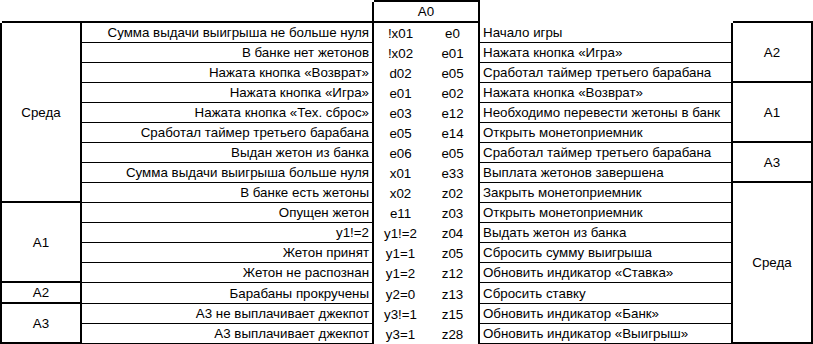
\includegraphics[width=\textwidth]{images/a0_pins.png}
\caption{Входные и выходные события автомата $A_0$.}
\end{figure}

\clearpage
\subsection*{Автомат 2. «Монетоприемник» ($A_1$)}

\begin{figure}[h]
\centering
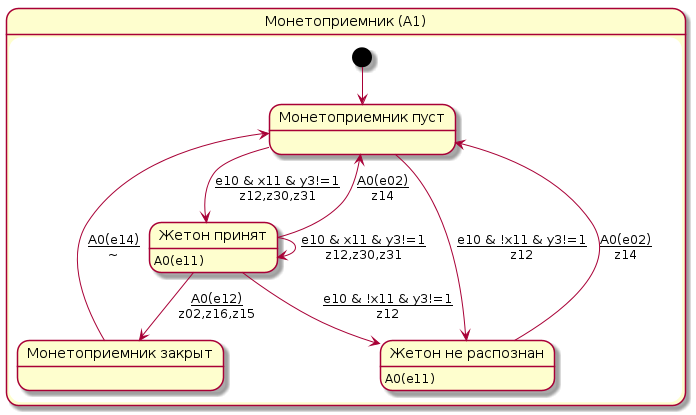
\includegraphics[width=0.8\textwidth]{images/a1_diagram.png}
\caption{Диаграмма состояний автомата $A_1$.}
\end{figure}

\begin{figure}[h]
\centering
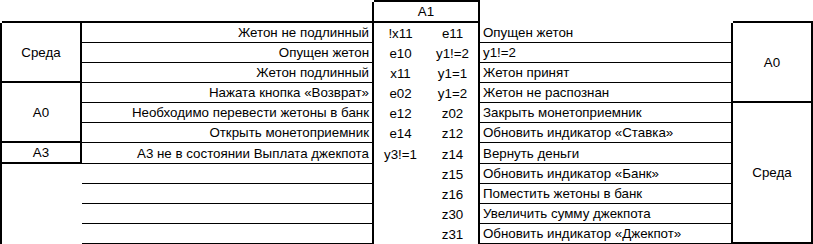
\includegraphics[width=0.9\textwidth]{images/a1_pins.png}
\caption{Входные и выходные события автомата $A_1$.}
\end{figure}

\subsection*{Автомат 3. «Игровые барабаны» ($A_2$)}

\begin{figure}[h]
\centering
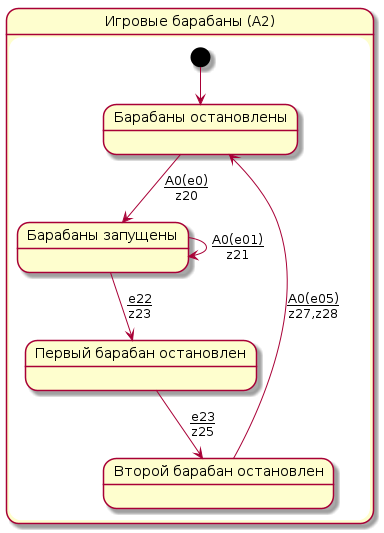
\includegraphics[width=0.55\textwidth]{images/a2_diagram.png}
\caption{Диаграмма состояний автомата $A_2$.}
\end{figure}

\begin{figure}[h]
\centering
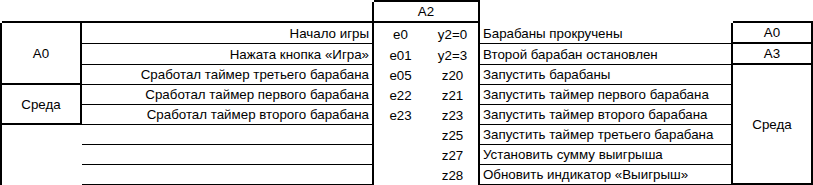
\includegraphics[width=0.8\textwidth]{images/a2_pins.png}
\caption{Входные и выходные события автомата $A_2$.}
\end{figure}

\clearpage
\subsection*{Автомат 4. «Джекпот-счетчик» ($A_3$)}

\begin{figure}[h]
\centering
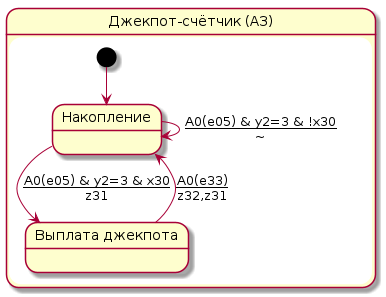
\includegraphics[width=0.55\textwidth]{images/a3_diagram.png}
\caption{Диаграмма состояний автомата $A_3$ --- нового вложенного автомата.}
\end{figure}

\begin{figure}[h]
\centering
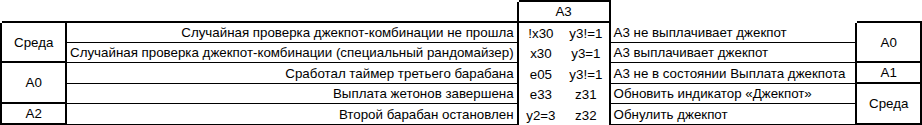
\includegraphics[width=0.9\textwidth]{images/a3_pins.png}
\caption{Входные и выходные события автомата $A_3$. Обратите внимание, что
  входы включают опрос состояния соседа \texttt{y2=3} автомата $A_2$
  --- то самое обращение к внутреннему состоянию второго вложенного
  автомата, ради которого дорабатывался алгоритм.}
\end{figure}

\clearpage
\section{Итоговый перемноженный автомат}

\begin{figure}[h]
\centering
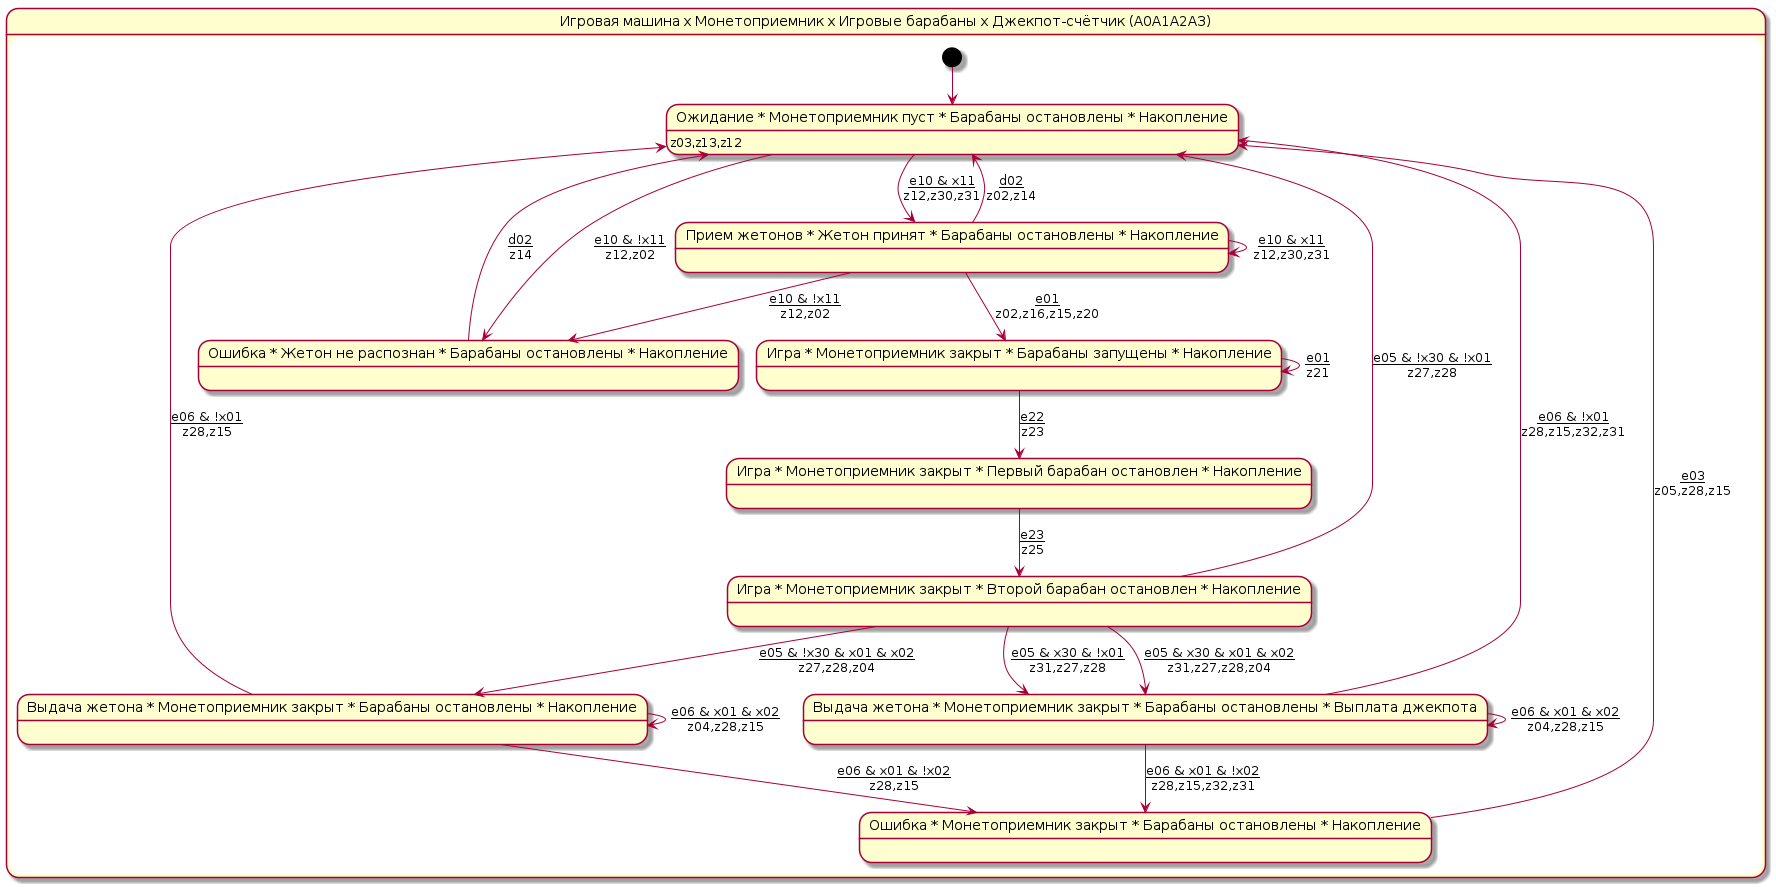
\includegraphics[width=\textwidth]{images/final_diagram.png}
\caption{Диаграмма состояний итогового автомата
  $A_0\times A_1\times A_2\times A_3$.}
\end{figure}

\begin{figure}[h]
\centering
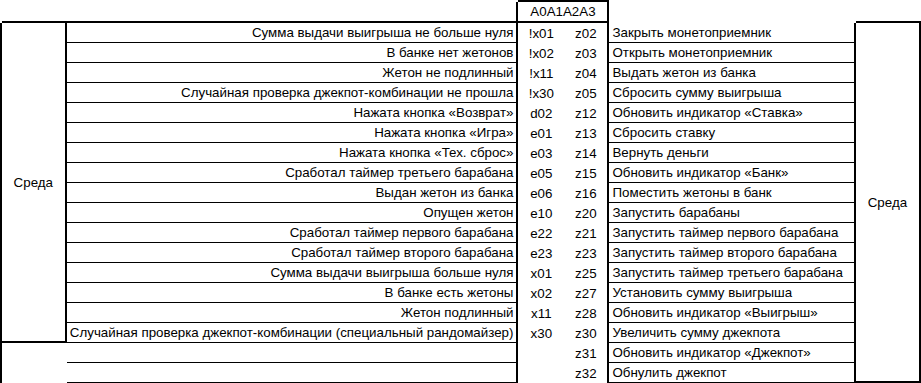
\includegraphics[width=\textwidth]{images/final_pins.png}
\caption{Входные и выходные события итогового автомата.}
\end{figure}

\clearpage
\section*{Вывод}

Новый вложенный автомат добавил всего лишь одно новое состояние, а не
увеличил итоговый автомат в несколько раз. Это позволило всё так же
понимать, что происходит в итоговом перемноженном автомате.

\end{document}
